%% LyX 2.3.3 created this file.  For more info, see http://www.lyx.org/.
%% Do not edit unless you really know what you are doing.
\documentclass[11pt,a4paper,english]{desearticle}
\usepackage{mathptmx}
\usepackage{helvet}
\usepackage{courier}
\renewcommand{\familydefault}{\rmdefault}
\usepackage[latin9]{inputenc}
\usepackage{fancyhdr}
\pagestyle{fancy}
\usepackage{float}
\usepackage{booktabs}
\usepackage{graphicx}

\makeatletter

%%%%%%%%%%%%%%%%%%%%%%%%%%%%%% LyX specific LaTeX commands.
\pdfpageheight\paperheight
\pdfpagewidth\paperwidth

%% Because html converters don't know tabularnewline
\providecommand{\tabularnewline}{\\}

%%%%%%%%%%%%%%%%%%%%%%%%%%%%%% User specified LaTeX commands.
\Author{Vaibhav Shatalwar}
\Afil{DESE, IISc}
\Journal{Mechatronic Systems Design}
\Month{Aug-Dec}
\Year{2024}

\makeatother

\usepackage{babel}
\begin{document}
	\title{{\huge{}H-Bridge Control}}
	\maketitle
	\begin{abstract}
		The aim of experiment to understand use of L-298 bridge 
		by controlling using TIVA board. H-bridges are used in bidirectional motor drives.
	\end{abstract}
	
	\section{Introduction}
	In this experiment, we are using the L298 motor driver to control inductive loads, including relays, solenoids, DC motors, and stepper motors. The L298 is a monolithic integrated circuit available in 15-lead Multiwatt and PowerSO20 packages. It features two enable inputs that allow for independent control of the device, regardless of the input signals. The emitters of the lower transistors in each bridge are interconnected, and the corresponding external terminal can be utilized for the connection of an external sensing resistor \cite{L298N}.
	
	\section{Tasks}
	The experiment consists of several tasks, outlined as follows:
	
	\begin{itemize}
		\item Setup of the TIVA board
		\item Configuration of the L298N motor driver
		\item Development of a PWM program to drive the L298N
		\item Placement of resistors across the H-bridge and testing the circuit
	\end{itemize}
	
	\subsection*{TIVA Board Setup}
	The TIVA board, in conjunction with Code Composer Studio (CCS) available from ti.com, offers a user-friendly development environment. CCS seamlessly integrates with the Arm GNU Compiler (GCC), facilitating the compilation of C code and its execution on the TIVA board.
	
	\subsection*{L298N Setup}
	Since the L298 motor driver does not include internal diodes, external diodes must be added to the circuit. Additionally, external decoupling capacitors are necessary for both the logic and load supply. Figure \ref{fig:label1} illustrates the internal schematic of the H-bridge.
	
	\begin{figure}[!htbp]
		\centering
		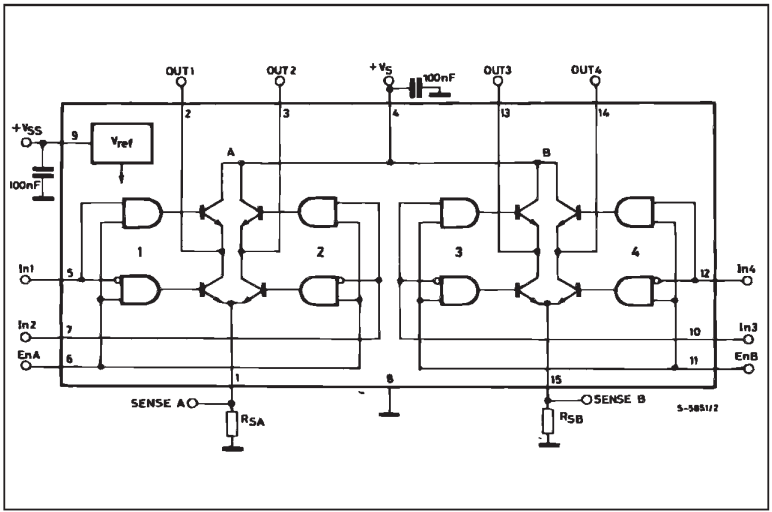
\includegraphics[width=0.8\linewidth]{img/sch_l298}
		\caption{\label{fig:label1}Logic Block Diagram of L298N \cite{L298N}}
	\end{figure}
	
	\subsection*{PWM Program to Drive L298N}
	A PWM (Pulse Width Modulation) program is developed to control the L298N motor driver.
	
	\subsection*{Place Resistors Across the Bridge and Test}
	For testing the circuit, a 10 ohm, 10 watt dummy load resistor is used. PWM signals are generated using a signal generator, and the duty cycle is varied. The voltage across the load resistor is observed on an oscilloscope. In Figure \ref{fig:label4}, a pulse with a $60\%$ duty cycle is applied, and the corresponding voltage across the load resistor is shown in Figure \ref{fig:label5}.
	
	\begin{figure}[!htbp]
		\centering
		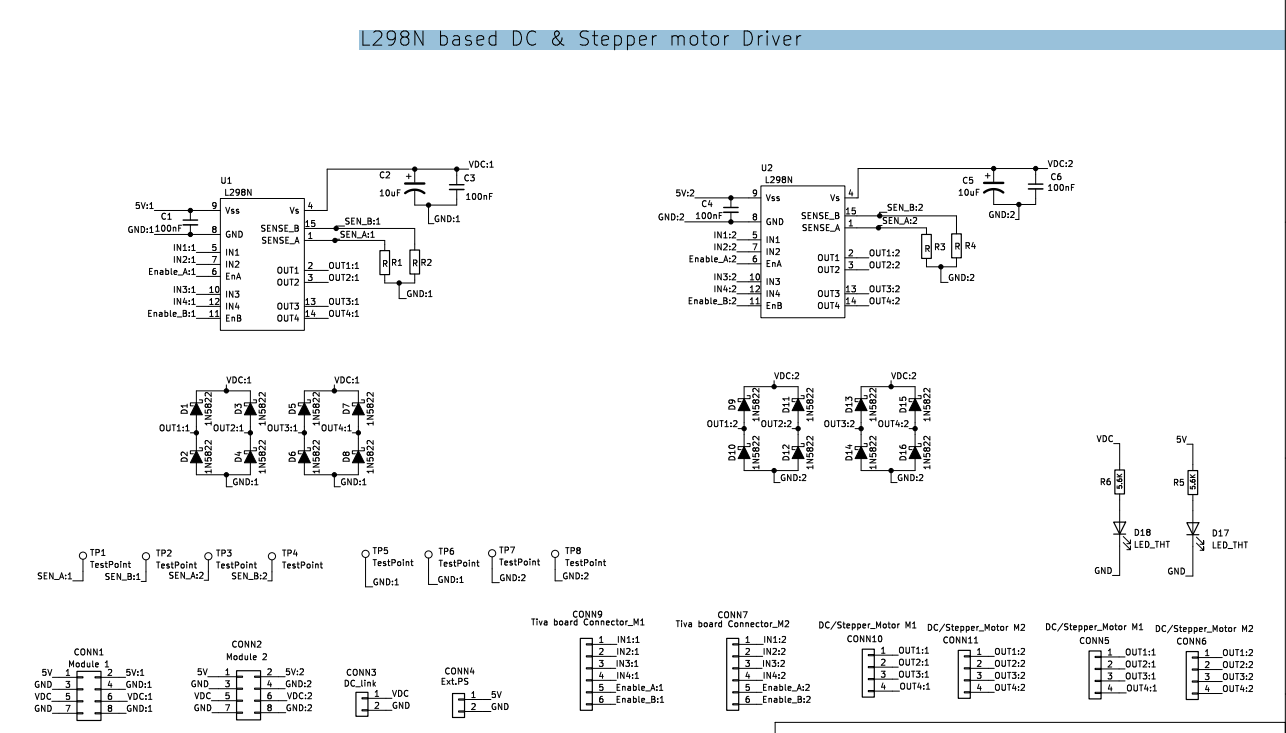
\includegraphics[width=0.8\linewidth]{img/sch_l298n}
		\caption{\label{fig:label2}Schematic of L298N H bridge driver board}
	\end{figure}
	
	\begin{figure}[!htbp]
		\centering
		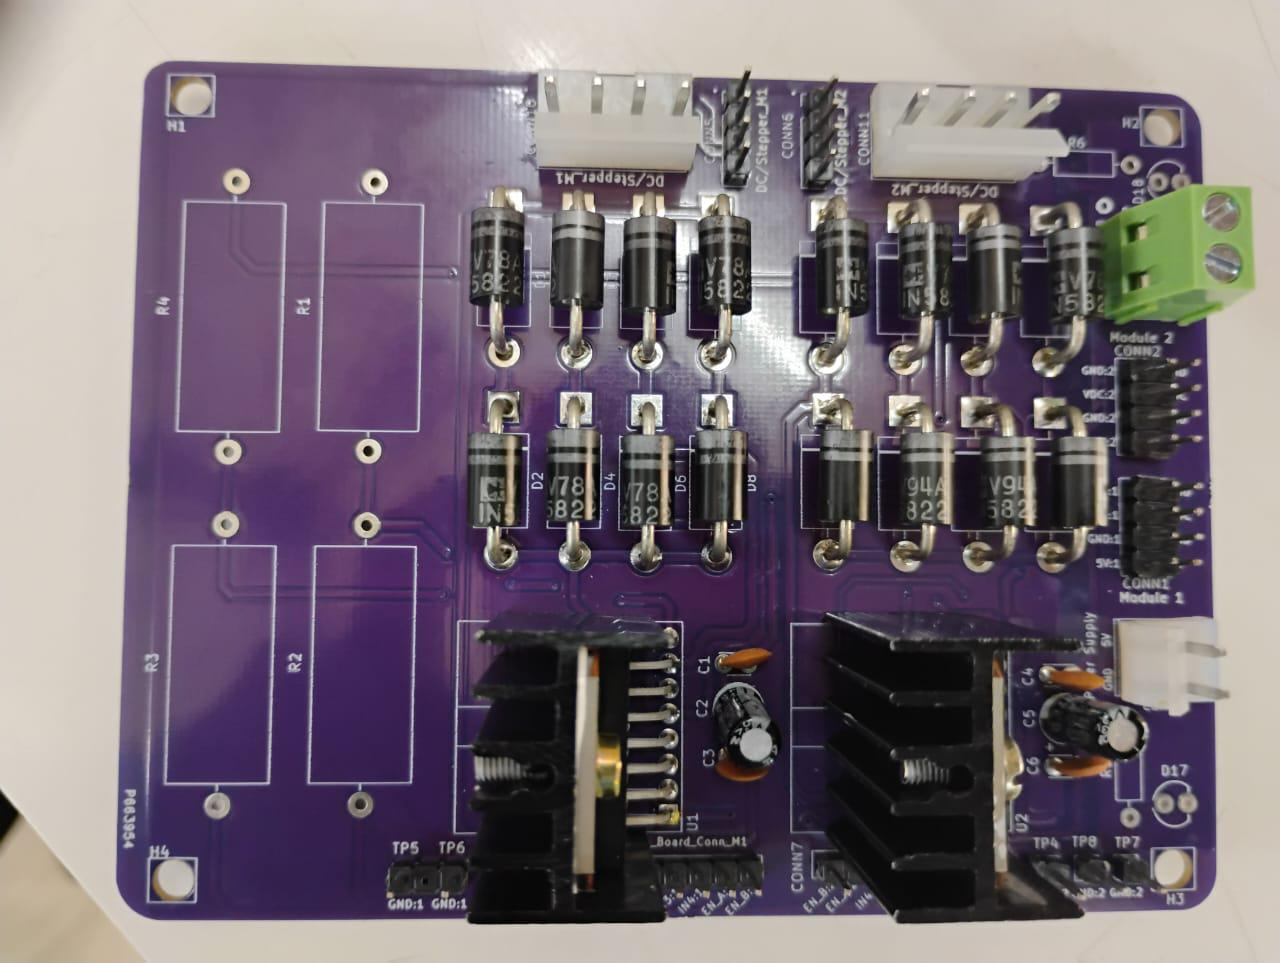
\includegraphics[width=0.8\linewidth]{img/pcb}
		\caption{\label{fig:label3} L298N H bridge driver board}
	\end{figure}
	
	\begin{figure}[!htbp]
		\centering
		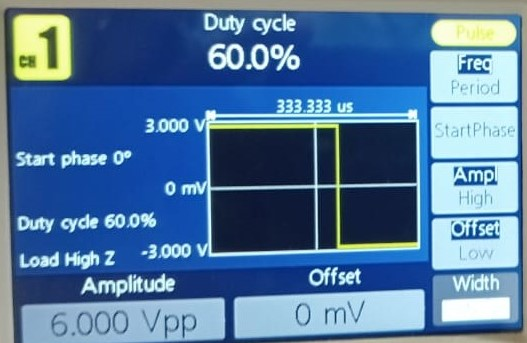
\includegraphics[width=0.8\linewidth]{img/set_1_1}
		\caption{\label{fig:label4} PWM signal from source generator with duty cycle $60 \%$}
	\end{figure}
	
	\begin{figure}[!htbp]
		\centering
		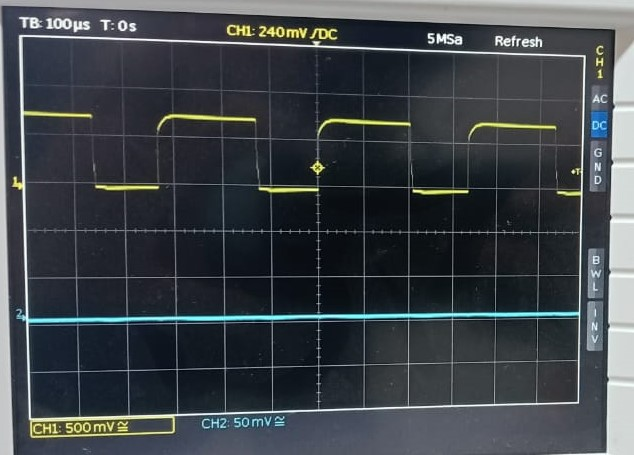
\includegraphics[width=0.8\linewidth]{img/set_1}
		\caption{\label{fig:label5} Voltage observed across load resistor}
	\end{figure}
	
	\begin{figure}[!htbp]
		\centering
		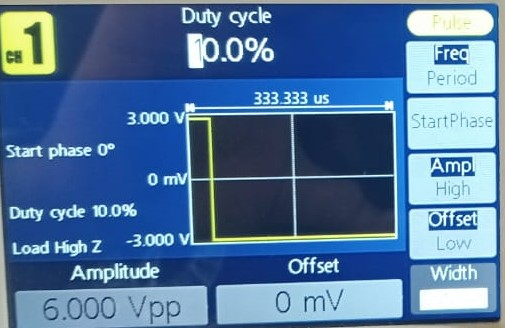
\includegraphics[width=0.8\linewidth]{img/set_2_1}
		\caption{\label{fig:label6} PWM signal from source generator with duty cycle $10 \%$}
	\end{figure}
	
	\begin{figure}[!htbp]
		\centering
		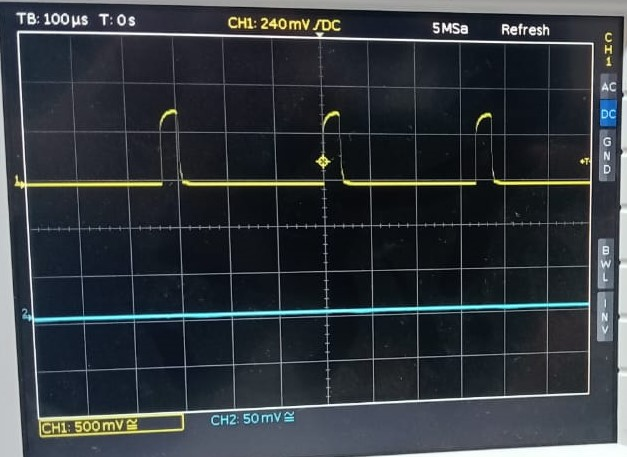
\includegraphics[width=0.8\linewidth]{img/set_2}
		\caption{\label{fig:label7} Voltage observed across load resistor}
	\end{figure}
	
	\begin{figure}[!htbp]
		\centering
		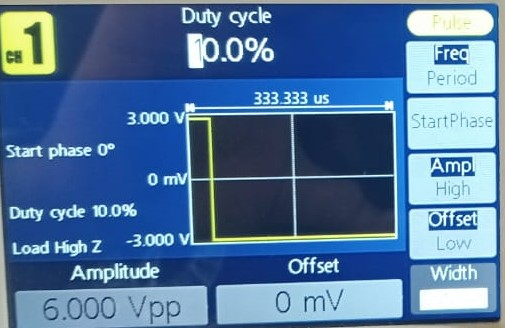
\includegraphics[width=0.8\linewidth]{img/set_2_1}
		\caption{\label{fig:label8} PWM signal from source generator with duty cycle $40 \%$}
	\end{figure}
	
	\begin{figure}[!htbp]
		\centering
		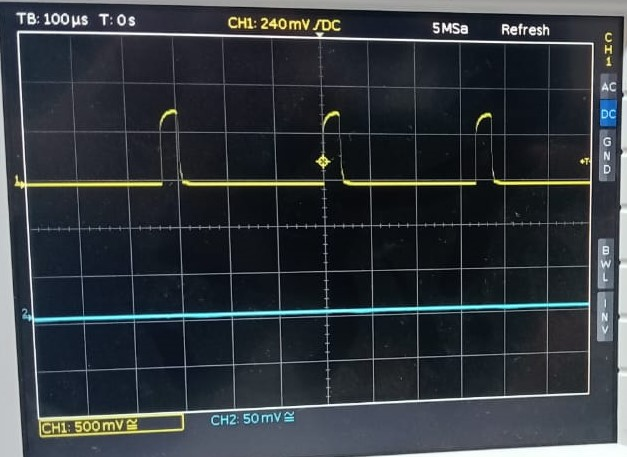
\includegraphics[width=0.8\linewidth]{img/set_2}
		\caption{\label{fig:label9} Voltage observed across load resistor}
	\end{figure}
	
	\section{Conclusions}
	In all cases, there was a slight variation in voltage across the load resistor, i.e., not a perfect PWM. This may be due to parasitic capacitance.

%In most cases, the experimental results will not match theoretical
%calculations. This sections addresses this by discussion on these
%mismatches. This is a very important section. It provides an insight
%into the authors' thought flow. Note that this section is not merely
%a summary of the entire article. It discusses the experiment from
%the angle of practicalities and uncertainities. As there are no ideal
%situations in practical realisations, the authors should discuss on
%aspects where the result is not as expected by theory. In what ways
%the short comings in the theory can be addressed? What are the possible
%solutions? Brainstorming is an essential component of this section.
%The authors can also put forth comparisons based on similar circuits,
%simulation results and discussions in literature to consolidate the
%results that have been obtained in this experiment.

\bibliographystyle{unsrt}
\bibliography{report}

\end{document}
